\documentclass[11pt]{amsart}
\usepackage{geometry}                % See geometry.pdf to learn the layout options. There are lots.
\geometry{letterpaper}                   % ... or a4paper or a5paper or ... 
%\geometry{landscape}                % Activate for for rotated page geometry
%\usepackage[parfill]{parskip}    % Activate to begin paragraphs with an empty line rather than an indent
\usepackage{graphicx}
\usepackage{amssymb}
\usepackage{epstopdf}
\usepackage{listings}
\usepackage{textcomp}
\lstset{language=Python,breaklines=true,upquote=true,commentstyle=\normalsize}
\DeclareGraphicsRule{.tif}{png}{.png}{`convert #1 `dirname #1`/`basename #1 .tif`.png}

\title{Phase-resolved Wave Prediction from a SWIFT Buoy Array}
\author{Michael Schwendeman}
\date{30 April, 2017}                                           % Activate to display a given date or no date

\begin{document}
\maketitle
\section{Introduction}
This project is motivated by a long-standing problem in wave-energy generation.  It is known that wave energy converters (WECs) can produce significant gains in efficiency by using advanced control techniques.  However, such techniques often require advanced knowledge of the incoming waves.  In the ideal case, the system is given an exact trace of the future wave excitation force.  As this is a difficult problem, most WECs are tuned instead based only on the average 30-minute bulk wave parameters. 

The goal of this project is to provide a useful prediction of the incident waves on a WEC, using an array of networked buoys.  By useful we mean that when coupled with advanced control techniques, the wave prediction improves upon the WEC performance over just using average wave parameters.
A related question, which may have widespread scientific applicability, is whether we can construct a realistic approximation of the sea surface from the sparse buoy array.

This report documents the progress made so far on these questions.  It is broken into three sections.  Section 2 outlines the integration of the SBG Ellipse IMU into the newest version (``v4") SWIFT buoys, and describes the Python program for receiving data in real-time using TCP-IP sockets and an RF ethernet bridge.  Section 3 details the development of a phase-resolved wave prediction algorithm using linear sea surface simulations of directional spectra.  Section 4 shows a preliminary evaluation of the phase-resolved algorithm using real data obtained from a research cruise off of Southern California.  As this is very much a work in progress, each section includes several recommendations and ideas for future work, which are together summarized at the end of the report.
%\subsection{}

\section{SBG and Ethernet Bridge Integration}

\subsection{System Overview}

A schematic of the buoy array approach to wave prediction is shown in Figure \ref{fig:WavePredictionSchematic}.  One of the major design considerations of the new SWIFT (surface wave instrument float with tracking) v4 drifters was their use in the wave prediction problem.  As in the version 3 SWIFTs, the SWIFT v4 is built around a Sutron Xpert microprocessor and data logger.  The Xpert has a 32-bit processor, supports SD memory, and has multiple serial and ethernet ports.  The Xpert logs the raw measurements from the SWIFT sensor payload, and performs onboard processing of certain data products.  These products are then transmitted over Iridium satellite communication to a server on land once per hour.

\begin{figure}[t]
    \centering
    \noindent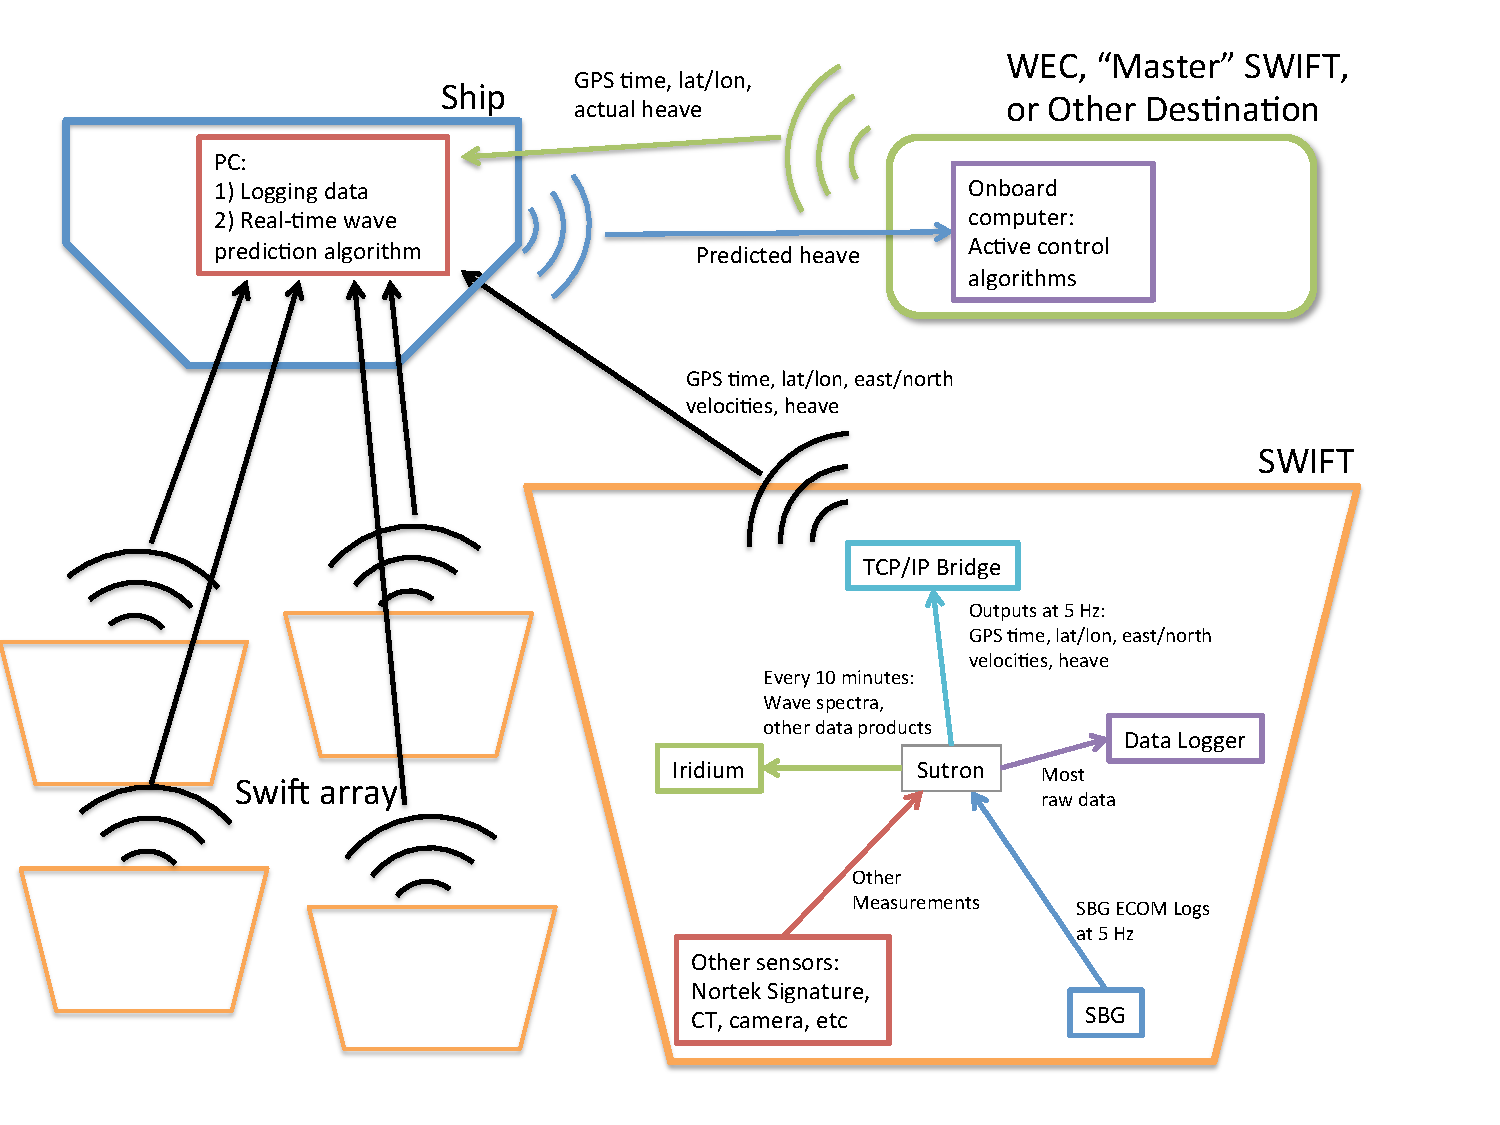
\includegraphics[width=5.5in]{WavePredictionSchematic.pdf}\\
   \vspace{-0in}\caption{Schematic showing the main components of the SWIFT buoy array and wave prediction architecture.}\label{fig:WavePredictionSchematic}
\end{figure}

The form factor of v4 buoys is significantly different than that of the previous SWIFTs, to accommodate the down-looking Nortek Signature 5-beam ADCP.  The v4 buoys no longer have the tall spar-type shape of the previous SWIFTs, which makes them slightly more susceptible to tipping motions.  Ballast was added to the buoy hulls below the water line to limit this effect, and drogues have been experimented with as well.  

For the purposes of this project, the most important change in the SWIFT architecture is the transition from a MicroStrain inertial package to one made by SBG Systems.  The SBG Ellipse-N is a miniature, high-performance MEMS based inertial system with an industrial GNSS receiver.  The Ellipse-N inertial motion unit (IMU) features three-axis gyroscopes, accelerometers, and magnetometers.  It also runs a real-time Extended Kalman Filter (EKF) for data fusion of its IMU and GPS measurements.  In combining the IMU and GPS data streams, the EKF uses the advantages of each measurement to produce a better position and orientation solution than from either measurement alone.  

The most critical measurement of the SWIFTs for real-time wave prediction is the buoy vertical position, or heave.  This is a difficult measurement because it requires two integrations of the inertial accelerometer signal, which leads to drift in the position.  At the same time, the accuracy of the GPS measurements is much worse in the vertical direction than horizontal.  To solve this problem, SBG have developed an advanced high pass filter specifically intended for estimating heave in real-time for marine purposes.  The filter is designed to limit phase and gain errors in wave motions with periods shorter than 15 seconds.

\subsection{SBG Ellipse Configuration and Magnetometer Calibration}
The SBG Ellipse-N is configured and calibrated using the sbgCenter application, which requires the device to be plugged in through serial or usb connectors.  sbgCenter allows you to set the output logs, connection settings, device orientation, lever arms, and aiding sensors (such as GPS).  The device saves its most recent configuration, so this step does not need to be repeated for each deployment.  Configuration settings are also saved and can be loaded from a file. See the dropbox SBG Systems folder in the SWIFT\_v4.x directory for the most up-to-date configuration.

One additional step is needed to ensure accurate measurements from the Ellipse, which is calibration of the internal magnetometer.  This is necessary because although the Ellipse comes calibrated from the factory, placing the Ellipse in the SWIFT puts it near components which may distort the magnetic field.  In this way the uncalibrated Ellipse heading measurement may be off by tens of degrees, which would seriously effect the accuracy of many of the necessary data products.  The calibration procedure is described in the Ellipse Hard \& Soft Iron Calibration Manual.  Unfortunately, the calibration uses the sbgCenter application, which requires the device to be plugged in to the computer.  Thus, the SWIFT cannot be fully sealed, which leaves open the possibility for small errors.  Caveats aside, the calibration procedure appears to bring the average heading error down from roughly 5\% or more to 1-2\%.

\subsection{Receiving SBG Data Over Ethernet Bridge}
The SBG Ellipse-N data is stored and transmitted as messages using the "sbgECom" binary protocol, as described in the Firmware Reference Manual.  The binary messages are logged to a file by the Xpert processor, and also transmitted asynchronously over a TCP/IP socket bridge.  The TCP/IP signal is then wirelessly transmitted over RF radio (900 MHz) via the Digi XPress Ethernet Bridge.  The XPress Ethernet Bridge has a stated range of 2-15 miles depending on the antenna used, and a data rate of 1.5 Mbps.  In Figure \ref{fig:WavePredictionSchematic}, the data from the SWIFT array and WEC (or other target point) are sent to a shipboard PC, where the prediction algorithm is run and returned to the WEC for active controls.  Alternatively, it may be preferable to have the algorithm running in an embedded system onboard the WEC.  

To stream data over the ethernet bridge to the PC, first follow the directions in the file Xpert\_EthernetBridge\_setup.txt.  This sets the IP addresses, Mac addresses, ports, etc. for both sides of the bridge --- namely the shipboard PC and Xpert microprocessor on the SWIFT.  To check that the Ethernet Bridge is setup properly, simply open a browser and navigate to the device IP address, where a screen will show statistics of the connection and device information, as shown in Figure \ref{fig:XpressBrowserInterface}.

\begin{figure}[t]
    \centering
    \noindent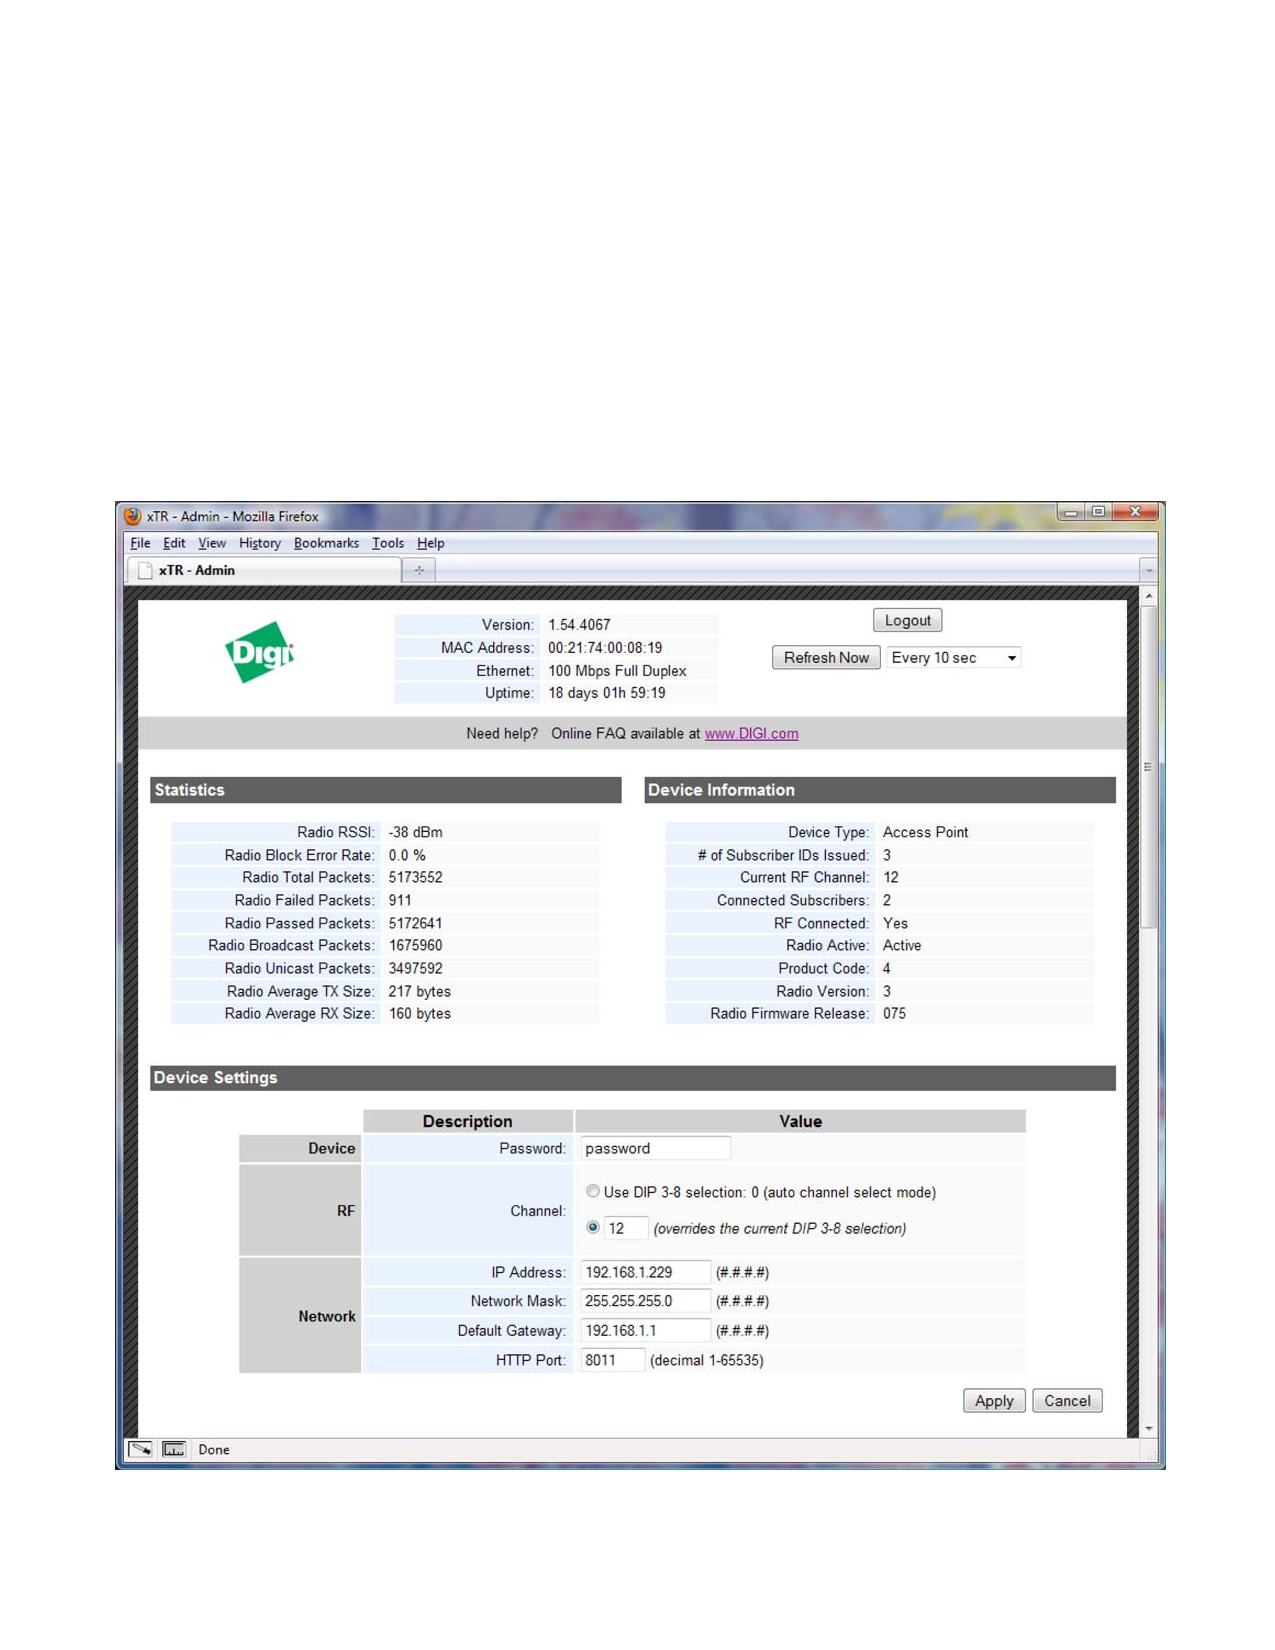
\includegraphics[width=5.5in]{XpressBrowserInterface.pdf}\\
   \vspace{-0in}\caption{Example of the Digi Xpress Ethernet Bridge browser interface.}\label{fig:XpressBrowserInterface}
\end{figure}


The software for receiving data from the SWIFTs and decoding the SBG binary messages is written in Python and contained in two files, which are outlined below. The file \texttt{readAndDecodeFromEthernetBridge.py} is a script which, when run from the PC, opens a TCP/IP socket, listens for incoming connections, and accepts data as available.  In this way, the PC acts as a server, in that it does not query for data, but accepts the data asynchronously.  The TCP/IP functionality is accessed through the Python socket module, which is available on all modern Unix, Windows, and MacOS platforms.  

As the data streams in, a series of if-statements check for the sync bytes that indicate the beginning of an sbgECom message, as detailed in the Ellipse Firmware Reference Manual.  When such a message is detected, the script calls a function \texttt{parseSbgMessage} which further decodes the binary data.  The parsing functions are accessed through the \texttt{sbgMessageParse} module contained in the file \texttt{sbgMessageParse.py}.  The function \texttt{\\parseSbgMessage} was written such that it can read binary data from a socket connection, as indicated above, or from a previously saved raw binary file.  In addition, it can print decoded data in ascii format to a file or to stdout.  The default behavior is to read the data from a socket connection and not print the output.

 A key piece of the parsing is the dictionary variable \texttt{sbgMessages}.  The \texttt{sbgMessages} dictionary contains all the information from the Firmware Reference Manual on the message ID, message name, message length (in bytes), field names, and field types (e.g. 8-bit unsigned integer, double float, etc.). For example, take the first entry:
 \begin{lstlisting}
b'\x01': {'name':'Status','intLength':22,'binLength': b'\x16\x00','unpackString':'<LHHLLLH','fields':('time_stamp','general_status','reserved1','com_status','aiding_status','reserved2','reserved3')
\end{lstlisting}
 This indicates that these message ID 1 (b`\textbackslash x01' in Python binary syntax) has name `Status,' length of 22 bytes (b`\textbackslash x16\textbackslash x00' in binary), and fields \texttt{`time\_stamp'} (unsigned 32 bit integer, or ``L"), \texttt{`general\_status'} (unsigned 16 bit integer, or ``H"), etc.  All of this information is taken from the Ellipse Firmware Reference Manual.  Thus, it is possible to add entries to the \texttt{sbgMessages} dictionary if new SBG messages are required at a later time. 
  
The function \texttt{parseSbgData} is called by the wrapper function \texttt{parseSbgMessage}, and is responsible for actually translating the binary messages into a usable Python data structure.  The code is quite compact:
 \begin{lstlisting}
### Function for parsing binary SBG messages into dictionaries     
def parseSbgData(msgID,binData):
    parsedData = struct.unpack(sbgMessages[msgID]['unpackString'],binData)
    dataStruct = OrderedDict(zip(sbgMessages[msgID]['fields'],parsedData))
    return dataStruct
\end{lstlisting}
 It uses the unpack function of the struct library to translate the message bytes into a tuple of integers and floats, as defined in the \texttt{unpackString} of the \texttt{sbgMessages} dictionary. Then, it puts those values into an ordered dictionary with the field names for that message type, also defined in the \texttt{sbgMessages} dictionary.  This \texttt{dataStruct} ordered dictionary is the final result of the parsing and is returned and/or printed.  The Python ordered dictionary works just like a regular dictionary except that when printed, the fields are always in order (i.e. with \texttt{time\_stamp} always printing first).

 
Finally, it should be noted that streaming and decoding of the SBG data could alternatively have been performed using C++.  Specifically, C comes with its own sockets library, and SBG provides an API, written in C++, which can decode the binary messages.  Python was used as it provided a more user-friendly approach, more online support, and easier debugging.  Additionally, a similar decoder was written in Matlab (function \texttt{sbgBinaryToMatlab.m} and script \texttt{sbgBinaryToMatlab\_Batch.m}) for use with logged binary files.  For example, these Matlab functions are used to decode the binary data for testing the prediction algorithm in Section 4.

\subsection{Future Work}

Some additional work is needed to operationalize the above procedure.  Notably, the Ethernet Bridge has not been tested in long range outside, and has not been installed permanently on the SWIFT hulls.  The system has been tested in the laboratory however, and works well to capture and decode SBG data from a single SWIFT over the Ethernet Bridge.  

The \texttt{readAndDecodeFromEthernetBridge.py} program needs to be written to accommodate multiple SWIFTs.  This may be slightly tricky, as the current script is quite linear.  It seems that rather than wait for one connection, it could be modified to wait for four (or as many SWIFTs are in use).  Meanwhile, in the \texttt{while True} loop, it could receive bytes from each connection and parse them one after another.  However, this flow has not yet been tested.  Alternatively, a more complex program would make use of the asynchronous processing modules available in Python, such as \texttt{asynchio}.

A helpful feature of the system is that data is saved in a buffer until the PC is ready to receive the data, so bytes are not lost.  Along the same lines, one feature that has not been implemented is a cyclic redundancy check (CRC), which can be used to look for dropped bytes in the data.  The outline of such a function is given in the SBG Firmware Reference Manual.

With the above modifications, the system will be able to run on a shipboard PC or embedded system onboard a WEC, allowing it to receive, parse, and save timestamped location and heave data from multiple SWIFTs over the RF Ethernet Bridge.  At which point, the next step will be to implement an algorithm which takes in that data, and outputs a prediction (in real time) of the incoming waves to the WEC.  The next sections outline the progress being made in the development of such an algorithm.

\section{Linear Simulations and Least Squares Prediction Algorithm}
- Recap Connell et al 2015 algorithm\\
- Show matlab algorithm.\\
- No data, want to simulate ocean waves.  Use WAFO toolbox seasim function.  Describe background.\\
- Two functions, one to calculate wave prediction at a point, one to make a gridded surface reconstruction.\\
- Input parameters: buoy number and array shape, target location or grid size and resolution, wave components and regularization parameter, time windows and delay\\
- Several examples.  Spectra source.  Buoy shape.  Buoy number.  Regularization and buoy components.  Time window.\\
- Runtime results\\
- Future work: constrain least squares solution based on directional wave spectra.  Systematic analysis of parameter relationships to errors.  More realistic simulations - currents, nonlinearity. \\

\section{Evaluation from SWIFT data}
- Describe LC-DRI experiment.\\
- Example SWIFT wave prediction.\\
- Envelope calculations.\\
- Examine surface reconstruction.\\
- Future work: rolling algorithm with incrementation, use velocity data\\

\section{Summary of Future Work}
- So far IO software integration and algorithm development progressed separately.  \\
- Hardware and IO integration could be ready for testing soon. Runs successfully on laboratory PC.  Has not been tested oustide, running on embedded system, with buoys at long range.  Currently only written for one buoy.  \\
- Algorithm development could use work.  Rolling estimator constrained by directional spectra would help against over-fitting to high frequencies and jumps between windows. Use of u,v velocities might be more accurate in field data. \\ 
- Systematic error analysis would be useful for informing future experiments.  How many buoys are needed and how close together must they be?   How to relate the distance between array and target to the time window and delay?

\end{document}  